\documentclass [11pt]{report}

\usepackage{fancyhdr}
\usepackage [french]{babel}

\usepackage[utf8]{inputenc}
\usepackage[T1]{fontenc}
\usepackage{textcomp}
\usepackage{graphicx}
\usepackage{titlepic}
\usepackage{boxedminipage}
\usepackage{listings}
\usepackage{minitoc}
\usepackage{footmisc}
\usepackage{color}

\pagestyle{fancy}



\title{
	
\includegraphics[scale=0.43]{images/Logojeu.png}
	 \\\vspace{20mm}
	\textbf{\Huge \itshape Cahier des charges }
	}




\author{ \\\vspace{2mm}
	Adrien Louge \\\vspace{2mm}
	Florent Youinou\\\vspace{2mm}
	Mathilde Laplaze\\\vspace{2mm}
	Thibault Gdalia\\\vspace{30mm}
	}



\date{17 janvier 2014}


\begin{document}

\renewcommand{\baselinestretch}{0.001}
\maketitle
\tableofcontents

\newpage
\chapter {Pr\'esentations}

	\section{ L'\'equipe }

		La Girafe est  un groupe constitué de quatre personnes : Adrien Louge alias "TiNyDGZz", le chef de ce projet, Mathilde Laplaze alias "Mattou", la seule fille du groupe, Florent Youinou alias "T4ze" et Thibault Gdalia alias "Skeat". Retenez bien ces pseudos car dans le reste de ce Cahier des Charges nous n'utiliserons plus nos noms et pr\'enoms. Nous sommes r\'epartie sur deux classes : la SUPB2 et la SUPD2.  \'Etant donné que le groupe compte deux redoublants, TiNyDGZz et Skeat, qui ont d\'eja eu cette configuration de groupe l'ann\'ee derni\`ere, nous savons qu'il n'est pas impossible de travailler entre \'el\`eves de classes diff\'erentes. Le groupe a \'et\'e form\'e en fonction des affinit\'es, ainsi que des comp\'etences de chacun que nous avons pu observer durant le premier semestre. Pour une meilleure ambiance dans l'\'equipe, et pour avoir un bon rythme de travail, le groupe s'est constitué de membres qui ont la volont\'e de travailler. 
	
	
	
	\newpage

	\section { Les Membres }
		\subsection {Mathilde "Mattou" Laplaze}
			blabla\\\vspace{10mm}
	
		

		\subsection {Adrien "TiNyDGZz" Louge}
			TiNyDGZz ou Adrien LOUGE, c'est moi même. Je me présente, 19 ans, bientôt 20 (vieux mec quoi..). Comme vous devez le savoir ou pas d'ailleur, je suis redoublant. En effet, l'envie de rester dans cette école et de revoir des professeurs comme Krisbool ou Gollum était trop intense, je n'ai donc pas pu m'empecher de revenir.\\
			 L'année précédente j'étais accompagner de Skeat pour le projet, de ce fait, étant lui aussi redoublant et ayant l'habitude de travail de groupe ensemble, nous avons décidé de nous remettre ensemble et d'embaucher T4ze et Mattou pour donner naissance à notre projet.\\
			 Étant énormément motivé et ayant des idées de jeux assez concrètes, j'ai ainsi décidé de prendre les choses en mains et de proposer des idées, de ce fait, les qutres membres du groupe ont décidés de me nommer chef de projet\\
			 J'ai deux frères qui sont sortis d'école d'ingénieur en informatique et qui maintenant ont le moyen de se payer des plaisir personnels, c'est la principale motivation a mon entrée a EPITA. Plus sérieusement l'envie d'apprendre à organiser un projet, à coder des logiciel, à innover font parti de mes plus grandes motivations. Et l'école me permet de réaliser toutes ces envies. Malgré les difficultés de l'année passée j'ai su me réadapter pour pouvoir démarrer cette année sur les chapeaux de roue. \\
			 L'année dernière je me suis concentré seulement sur le graphique et le code à été mit de côté. Cette année j'ai pris la décision de faire les deux !\\\vspace{10mm}
	
\newpage 

		\subsection {Florent "T4ze" Youinou}
		T4ze, c’est moi. \'Etant fils d’ingénieur en informatique, ma passion me vient de mon père et contrairement aux enfants de mon âge, je n’ai jamais été un grand fan des jeux vidéo. Ainsi pendant que les autres s’amusaient sur leur console, moi je bidouillais sur mon ordinateur. J’ai donc commencé tôt à coder. Connaissant mes ambitions je me suis très vite investit dans les études qui me permettrait d’y accéder. Le problème c’est que du coup pour moi, les autres matières étaient totalement inutile et me faisait perdre mon temps. J’ai donc suivi passé un bac S SI (Science de l’Ingénieur) avec la spé ISN. J’adore apprendre et écouter les suggestions construites de personnes extérieurs.\\
\indent Mais l’idée de vivre accroché à un siège devant un écran ne donne pas envie, heureusement j’ai d’autres passions pour me changer les idées. En effet je fais beaucoup de sport, je sors souvent et ma plus grande source d’inspiration pour coder me vient des films que je regarde.\\\vspace{10mm}

	
		
		
		\subsection {Thibault "Skeat" Gdalia}

			Moi c'est Skeat, je suis en SUP a EPITA pour la deuxi\`eme fois (oui j'ai redoubl\'e),  c'est donc mon deuxi\`eme projet, l'ann\'ee derni\`ere au sien du groupe DAMNIT. Cette ann\'ee je suis toujours motiv\'e pour travailler en groupe, et accro\^itre mes comp\'etences en C\# . 
			\\ \indent  Avant de rentrer \'a EPITA, j'ai fait une terminal S Sciences de l'Ing\'enieur, depuis que je suis en prem\'iere je code, j'ai commenc\'e par le Visual BAsic en cours au lyc\'ee puis je me suis tourn\'e vers le C++. Je n'ai jamais \'et\'e un grand fan de jeu vid\'eo, j'ai toujours pr\'ef\'er\'e faire du sport ou sortir faire la f\^ete (donc rien a voir avec un GEEK). L'ann\'ee derni\`ere je n'ai pas valid\'e mon ann\'ee car je suis arriv\'e avec trop de lacune, mais cette ann\'ee va \^etre une autre histoire, c'est pour cela que j'ai choisi de faire parti de ce groupe qui \'a l'air tr\`es motiv\'e. De plus je connais tr\`es bien TiNyDGZz avec qui j'ai travaill\'e l'ann\'ee derni\`ere.\\\vspace{10mm}
	
	

\chapter{Principe et histoire du jeu}
	Dans le cadre de notre première année nous avons un projet à faire par groupe de quatre personnes. C'était donc pour nous un parfait moyen d'apprendre de facon ludique puisque nous avons décidé de faire un jeux vidéo.\\\\

\indent Nous sommes partis sur un jeu en 2D bas\'e sur un principe tr\`es connu, que l'on retrouve dans Jetpack ou encore Badland, tout en y apportant notre touche personnel. Le personnage doit parcourir les différentes maps du jeu, en évitant les nombreux obstacles se trouvant sur son chemin. Afin que le jeu est un peu plus d'interet pour le joueur, les maps devront être debloquées les unes à la suite des autres, et deviendront de plus en plus dur, avec de nouveaux obstacles.

\indent Le joueur ne pourra pas déplacer son personnage comme il le souhaite, il pourra juste lui faire faire un bond en appuyant sur espace (jusque la rien de bien nouveau). En plus de cela il devra manger les bonbons qui se trouvent sur son chemin afin de faire remonter sa barre d'energie. \`A chaque fois que le joueur touche un obstacle il est ralenti, chaque bond effectué par le personnage lui consomme de l'énergie. Pour regagner son énergie, le joueur à deux possibilitées : attendre que la barre se recharge avec le temps ou manger des bonbons. La partie est perdue si le personnage est ejecté de l'écran par la gauche. Cela peut arriver si le joueur se retrouve coincé par un obstacle. Si au contraire il parvient au bout de la map, la partie est remportée.
\newpage 


\chapter {Partage du travail}
\begin{center}
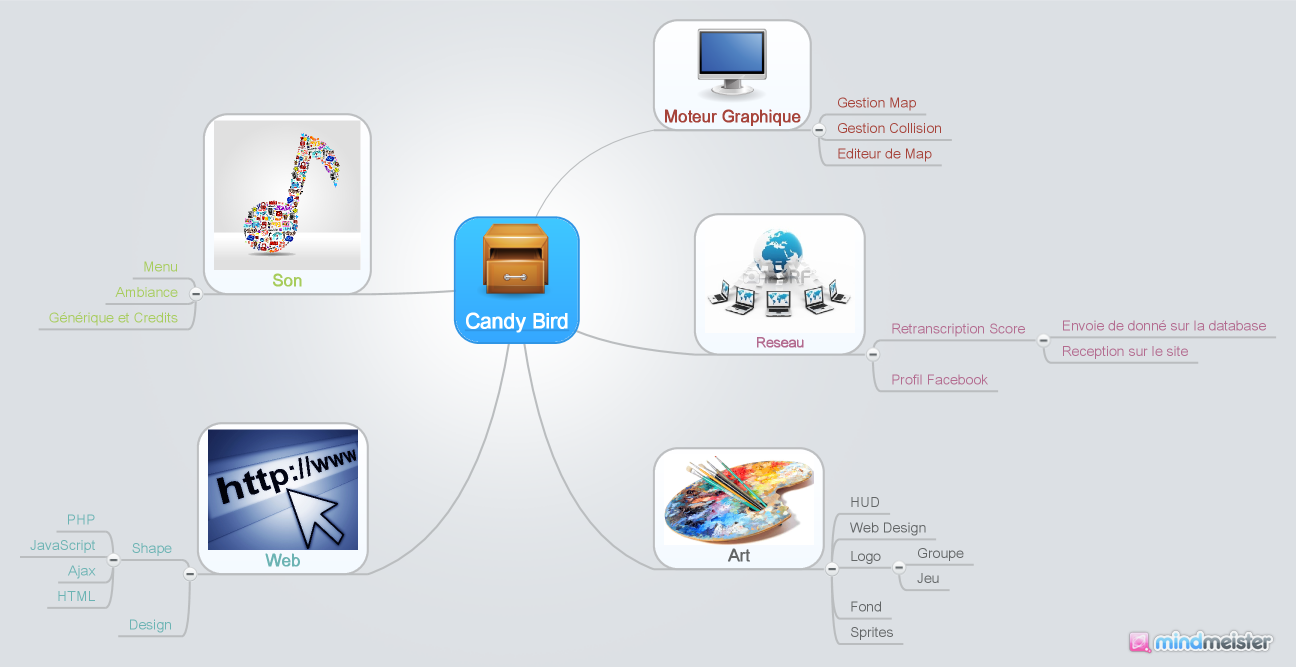
\includegraphics[scale=0.3]{images/Candy_Bird.png}
\end{center}

\newpage 

	\section{Repartitions}
		\subsection{Tâches}
			\begin{tabular}{| l |*{4} {c|}}
				\hline
				Themes & Mathilde & Adrien & Florent & Thibault \\
				\hline
				Son & X & & & X \\
				\hline
				Reseau & & & X & X \\
				\hline
				Site Internet & & & X & \\
				\hline
				Graphisme & X & X & & \\
				\hline
				Moteur Physique & & X & X & X\\
				\hline
			\end{tabular}\\\vspace{3mm}


		\subsection{Soutenances}
			\begin{tabular}{| l | * {3}{c|}}
				\hline
		 		& Soutenance 1 & Soutenance 2 & Soutenance 3 \\
				\hline
				Moteur Physique & 50\% & 75\% & 100\% \\
				\hline
				 Graphisme & 50\% & 80\% & 100\% \\
				\hline
				Réseaux & & & 100\% \\
				\hline
				Site internet & 50\% & 100\%  & 100\%  \\
	          			 \hline
				Son & 50\% & 80\% & 100\% \\
				\hline
				\'Editeur de map & 50\% & 100\% & 100\% \\
				\hline
			\end{tabular}\\\vspace{4mm}


	\section{Graphismes}
		\subsection {Logo}
			\paragraph{Jeu}
			L'idée de ce logo provient du célèbre jeu CandyCrush, et sa couleur Orangée/Marron s'inspire des sodas. Ces reflets clairs et ces bulles présentes un peu partout dans le titre rappellent le côté sucré d'un bonbon et annoncent ainsi en quelque sorte l'idée du jeux (un oiseau gourmand qui doit avaler des bonbons pour avoir des forces). 

			\paragraph{Groupe}
			Le logo de groupe quant à lui a été décidé assez au hasard. En effet, un jour Skeat et TiNy ont vu un Flashcode et se sont demandé pourquoi ne pas en faire le logo du groupe. Lorsque vous flashez le flashcode (Logique non ?) il vous amènera directement sur le site internet du projet, ce qui nous permet de nous faire connaitre implicitement. Pour ne pas avoir un simple flashcode noir et blanc, nous avons cherché à le personaliser et c'est ainsi que s'est crée notre logo. Pour rester dans les tons du jeux, sa couleur bleue a été choisie par rapport à la salopette bleue du petit oiseau principal !\\\vspace{5mm}

		\subsection {Fonds et obstacles}
 		Les fonds qui défilent ainsi que les obstacles sont installés avec une version par défaut mais pourront par la suite être modifiés en fonction de la période en cour. Par exemple un thème hiver, été, paques, noel, etc..\\\vspace{5mm}

		\subsection {Personnage(s)}
 		Pour rester fidèle au nom du jeux, CandyBird, le personnage officiel est donc un oiseau, et plus précisément un houla-houla.
 		Mais cet animal est loin d'être un oiseau ordinaire. En effet, à cause de la patie inférieure de son corps trop développée, il lui est difficile de voler pres du sol. De plus, c'est un animal gourmand et peu joyeux. Il a besoin d'avoir avaler une grande quantité de sucre pour pouvoir s'envoler.\\
Mais cet oiseau, tout comme les fonds, pourra être modifié dans des versions ultérieures du jeux et ainsi se transformer en d'autres espèces.\\\vspace{5mm}



	\section {Moteur Physique}
	Pour ce style de jeu le moteur physique est assez rudimentaire. Nous avons donc décidé de faire varier les lois de la physique d'une map à l'autre ou en même au cours d'une même map afin de rendre le jeu un peu plus dure et amusant. Ainsi, la vitesse de l'oiseau et la gravité ne seront pas constantes sur l'ensemble des maps. Toujours dans le but de rendre le jeu plus divertissant,le joueur n'aura pas la possibilité de faire descendre son personnage, il ne pourra qu'attendre le meilleur moment pour lui faire faire un bond.\\\vspace{5mm}



	\section {Réseaux}
	Afin de rendre le jeux plus interessant d'un point de vue social, l'idée nous est venu de mettre en place un système de classement. En ouvrant le jeux il nous sera donc possible de se connecter (à un compte créé auparavant) ou de jouer localement. Si l'on se connecte, en fin de partie notre score sera automatiquement envoyé sur le site officiel du jeux et s'affichera dans la catégorie classement. Cela permettra de comparer son score avec celui d'un ami, ou tout simplement de voir notre niveau par rapport à tous les joueurs.\\\vspace{5mm}


	\section {Menu}
	Un menu facilitera l'agencement des différents états du jeux. Dans le menu principale il sera possible de ce connecter à son compte à la seule condition que le joueur ai préalablement créer son profil via notre site internet ou directement depuis le jeux. Il sera aussi possible de naviguer depuis cle menu à travers les options du jeux ou l'on aura par exemple le choix entre activer ou désactiver le son du jeu ou encore régler la résolution du jeux afin t'optimiser l'affichage en fonction de son ordinateur. \`A tout moment l'utilisateur pourra bien évidement commencer une nouvelle partie. \\
\indent Durant une partie un menu pause sera disponible pour ne pas avoir à quitter entièrement le jeux, ou à perdre la partie losque l'on doit faire quelque chose entre temps. Dans ce menu, le joueur pourra : reprendre la partie, revenir au menu principal ou encore quitter le jeu.\\\vspace{5mm}


	\section {Communication}
	Pour permettre au jeux de se faire conna\^itre, et pour suivre son \'evolution, un site web sera mis en place. Une grosse partie du site sera dédiée aux nouveautés du jeux, aux presentations ainsi qu'aux rapports de soutenances. Une partie photo regroupera quelques clichés de nous travaillant sur le projet et des screen-shot du jeux. Un formulaire de contact sera disponible afin de nous faire part d'idée d'am\'eliorations, de bug, ou de tout commentaires relatif au jeux. Quand cette la gestion réseau sera opérationnelle nous mettrons aussi en place une page dédiée au classement des joueurs.
\\\\ \indent
	De plus, une page facebook sera ouverte à l'effigie de notre jeux. Car nous savons qu'il est plus simple de toucher un maximum de personnes par l'intermédiaire de ce réseau social. Nous y mettrons l'ensemble de nos actualités, les nouveauté sur le jeu, des images de notre travail afin d'interpeler les internautes. De plus il y sera tres simple de nous contacté quelqu'en soit la raison.

	\section {\'Editeur de Maps}
	Nous avons décidé de faire les maps dans des fichiers externes, sous formes de tableaux en associant des charactères spécifiques à chaque élément du décors. \'Etant donné que nous n'avons aucune envie d'écrire toutes les maps à la main, nous allons créer un éditeur de maps qui sera par la suite intégré au jeu. Ainsi, le joueur pourra lui même créer des niveaux et pourquoi pas les partager avec les autres joueurs pour les mettre au défis, ce qui nous permet d'allonger la durée de vie du jeu.\\\vspace{5mm}


	\section {Son}
	Un jeux, c'est bien, mais avec du son c'est mieux ! Nous allons utiliser une extension de XNA, Xact, qui nous permettra de g\'erer une biblioth\`eque de sons dans le jeux. Cette biblioth\`eque nous permettra d'am\'eliorer nos \'ev\'enements avec des musiques d'ambiances (sound sur Xact) et des effets sonores lors des actions du joueur (les sounds effects). Ainsi chaque événement lors d'une partie tel que les bons de l'oiseau ou encore lorsqu'il y a une collision entre l'oiseau et un élément du décor, sera accompagné d'un sound effect. Ainsi, toutes les maps auront leurs propres ambiances, par contre il n'y aura qu'une seule et même légère musique dans les menus. L'ensemble des sons seront récupéré sur internet car nous n'avons malheureusement pas de musiciens dans notre groupe donc nous feront avec ce que l'on trouvera. Puisque la musique n'est qu'une feature du jeux, il faut limiter son temps de recherche, nous ne seront donc que deux à travailler sur cette partie.



\chapter {Ressources utilisées}
	\section {Logiciels}

	Pour ce projet nous utiliserons plusieurs logiciels afin de programmer les différentes parties :\\

	- Notepad++ : Le site internet a quasiment été entierement codé à la main via cet éditeur de texte. Ainsi que les maps du jeu.\\\\\indent
	- Wamp : Pour pouvoir creer et tester le site en local.\\\\\indent
	- Visual Studio 2010 (avec XNA) : Afin de réaliser notre jeux en c\#, nous avons utilisé Visual Studio.\\\\\indent
	- Photoshop CS6 : La plupart des graphismes ont été réalisés à l'aide de Photoshop.\\\\\indent
	- TeXWork : Parce que écrire du \LaTeX sur le bloc note c'est pas simple.\\\vspace{10mm}



	\section {Autres}

	Pour apprendre/comprendre les différents langages de programmations dont nous nécessitions, nous avons utilisé de nombreux tutoriels. De même, il nous a fallut chercher sur internet comment utilisé les logiciels. Et comme la plupart du temps quand on a un probleme, on est pas le seul, les forums nous ont permit de corriger des bugs ou même améliorer notre code.


\chapter {Budget pour le projet}
	Nous avons fait une petite prévisions de nos dépense pour se projet :\\\\
				\begin{tabular}{|l|c|}
				\hline
		 		 & Prix \\
				\hline
				Ordinateur & 485 €  \\
				\hline
				 Serveur &  \\
				\hline
				Pizza / Kebab & Bcp  \\
				\hline
				Bière  & Bcp  \\
	          			 \hline
				Total & \\
				\hline
				
			\end{tabular}
\chapter {Conclusion}
	Ainsi nous avons poser les bases de notre projet, nous avons fixer les objectifs a atteindre pour chaque soutenance

\end {document}